\noindent The T-type attenuator (Fig. \ref{fig:tee-type-attenuator-schematic}) is the natural counterpart of the $\pi$-type attenuator. Its design equations can also be found in \cite{vizmuller1995rf}.


  \begin{figure}[ht]
    \centering
    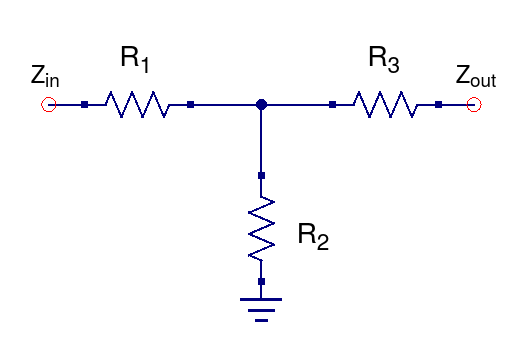
\includegraphics[width=5cm]{./images/tee-attenuator-schematic.png}
    \caption{T-type attenuator}
    \label{fig:tee-type-attenuator-schematic}
  \end{figure}
  
  \begin{equation}
  	R_{2} = \frac{2 \cdot \sqrt{Z_{in} \cdot Z_{out} \cdot 10^{\alpha/10}}}{10^{\alpha/10}-1}
  \end{equation}  
  
  \begin{equation}
  	R_{1} = \frac{10^{\alpha/10} + 1}{10^{\alpha/10} - 1} \cdot Z_{in} - R_2
  \end{equation}
  
    \begin{equation}
  	R_{3} = \frac{10^{\alpha/10} + 1}{10^{\alpha/10} - 1} \cdot Z_{out} - R_2
  \end{equation}
  
  
\noindent where $\alpha$ is the attenuation in dB. The power dissipated in each resistor can be derived using network analysis. Consider the node voltages and currents indicated in Fig. \ref{fig:power-dissipation-tee-type-attenuator} and let $P_{R1}$, $P_{R2}$ and $P_{R3}$ be the power dissipated by $R_1$, $R_2$ and $R_3$, respectively.

  \begin{figure}[ht]
    \centering
    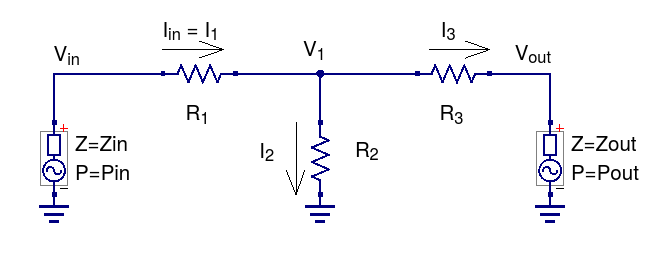
\includegraphics[width=10cm]{./images/tee-attenuator-power-dissipation.png}
    \caption{Node voltages and currents for the T-type attenuator}
    \label{fig:power-dissipation-tee-type-attenuator}
  \end{figure}
  
\noindent Then,
  
  \begin{equation}
  	P_{R1} = P_{in} \cdot \frac{R_1}{Z_{in}}
  \end{equation}
  
  \begin{equation}
  	P_{R2} = P_{in} \cdot  \frac{(R_1 - Z_{in})^2}{R_2 \cdot Z_{in}}
  \end{equation}
   
  \begin{equation}
  	P_{R3} = P_{in} \cdot \frac{R_3 \cdot (R_1 + R_2 - Z_{in})^2}{Z_{in} \cdot R_2^2}
  \end{equation}
  

 \noindent Fig. \ref{fig:pi-tee-relative-power-dissipation-50-Ohm} shows the relative power dissipation per resistance in a $\pi$ and $T$-type attenuators in a 50 $\Omega$ system. As shown, $R_1$ dissipates most of the power for attenuations greater than 6 dB and it dissipates more than the 90 \% of the power for attenuations greater than 27 dB. Please also notice that the power dissipation curves of the $\pi$ and T-type attenuators are the same as long as $Z_{in} = Z_{out}$. However, as shown in Fig. \ref{fig:pi-tee-relative-power-dissipation-50-75-Ohm} if $Z_{in} \neq Z_{out}$ the relative power dissipated at the resistors differs between the $\pi$ and the T-type attenuator.
 
   \begin{figure}[ht]
    \centering
    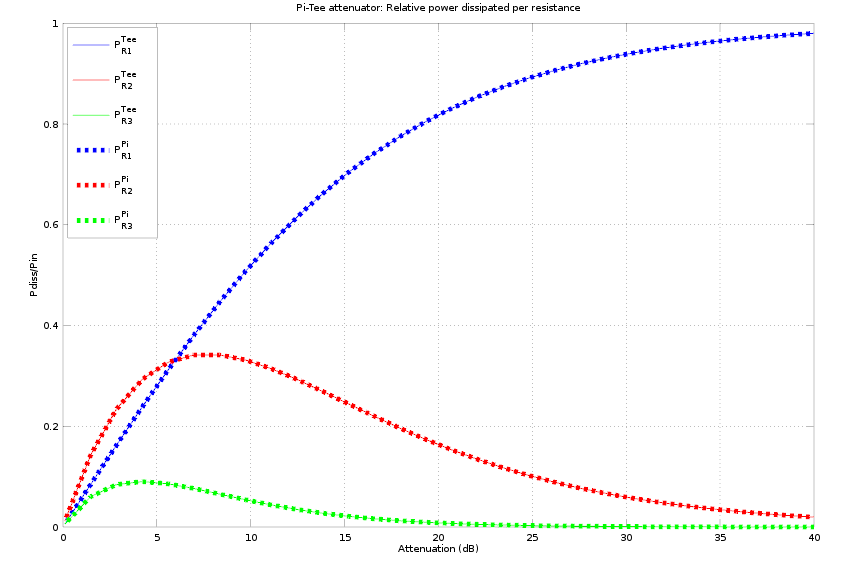
\includegraphics[width=10cm]{./images/pi-tee-relative-power-dissipation-50-Ohm.png}
    \caption{Power dissipated at the resistors in the $\pi$ and T-type attenuators relative to the input power. $Z_{in} = Z_{out} = 50 \Omega$}
    \label{fig:pi-tee-relative-power-dissipation-50-Ohm}
  \end{figure}
  
     \begin{figure}[ht]
    \centering
    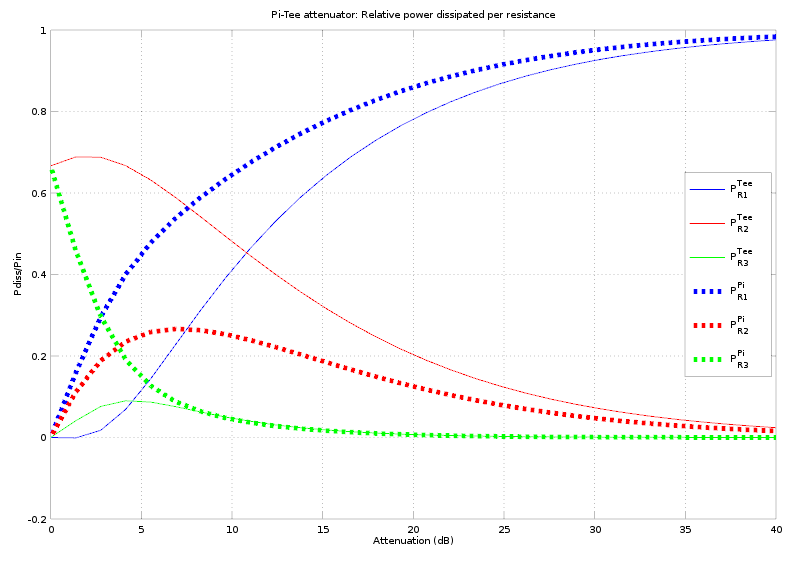
\includegraphics[width=10cm]{./images/pi-tee-relative-power-dissipation-50-75-Ohm.png}
    \caption{Power dissipated in the resistors for the $\pi$ and T-type attenuators with respect to the input power. $Z_{in} = 50 \Omega, Z_{out} = 75 \Omega$}
    \label{fig:pi-tee-relative-power-dissipation-50-75-Ohm}
  \end{figure}